\documentclass[convert={density=300,size=1080x800,outext=.png}]{standalone}
\usepackage{tkz-graph}
\usetikzlibrary{arrows,positioning,shapes,shapes.multipart,patterns,mindmap,shadows}
\usepackage{xcolor}
\usepackage{helvet}
\renewcommand{\familydefault}{\sfdefault}


\begin{document}

\footnotesize
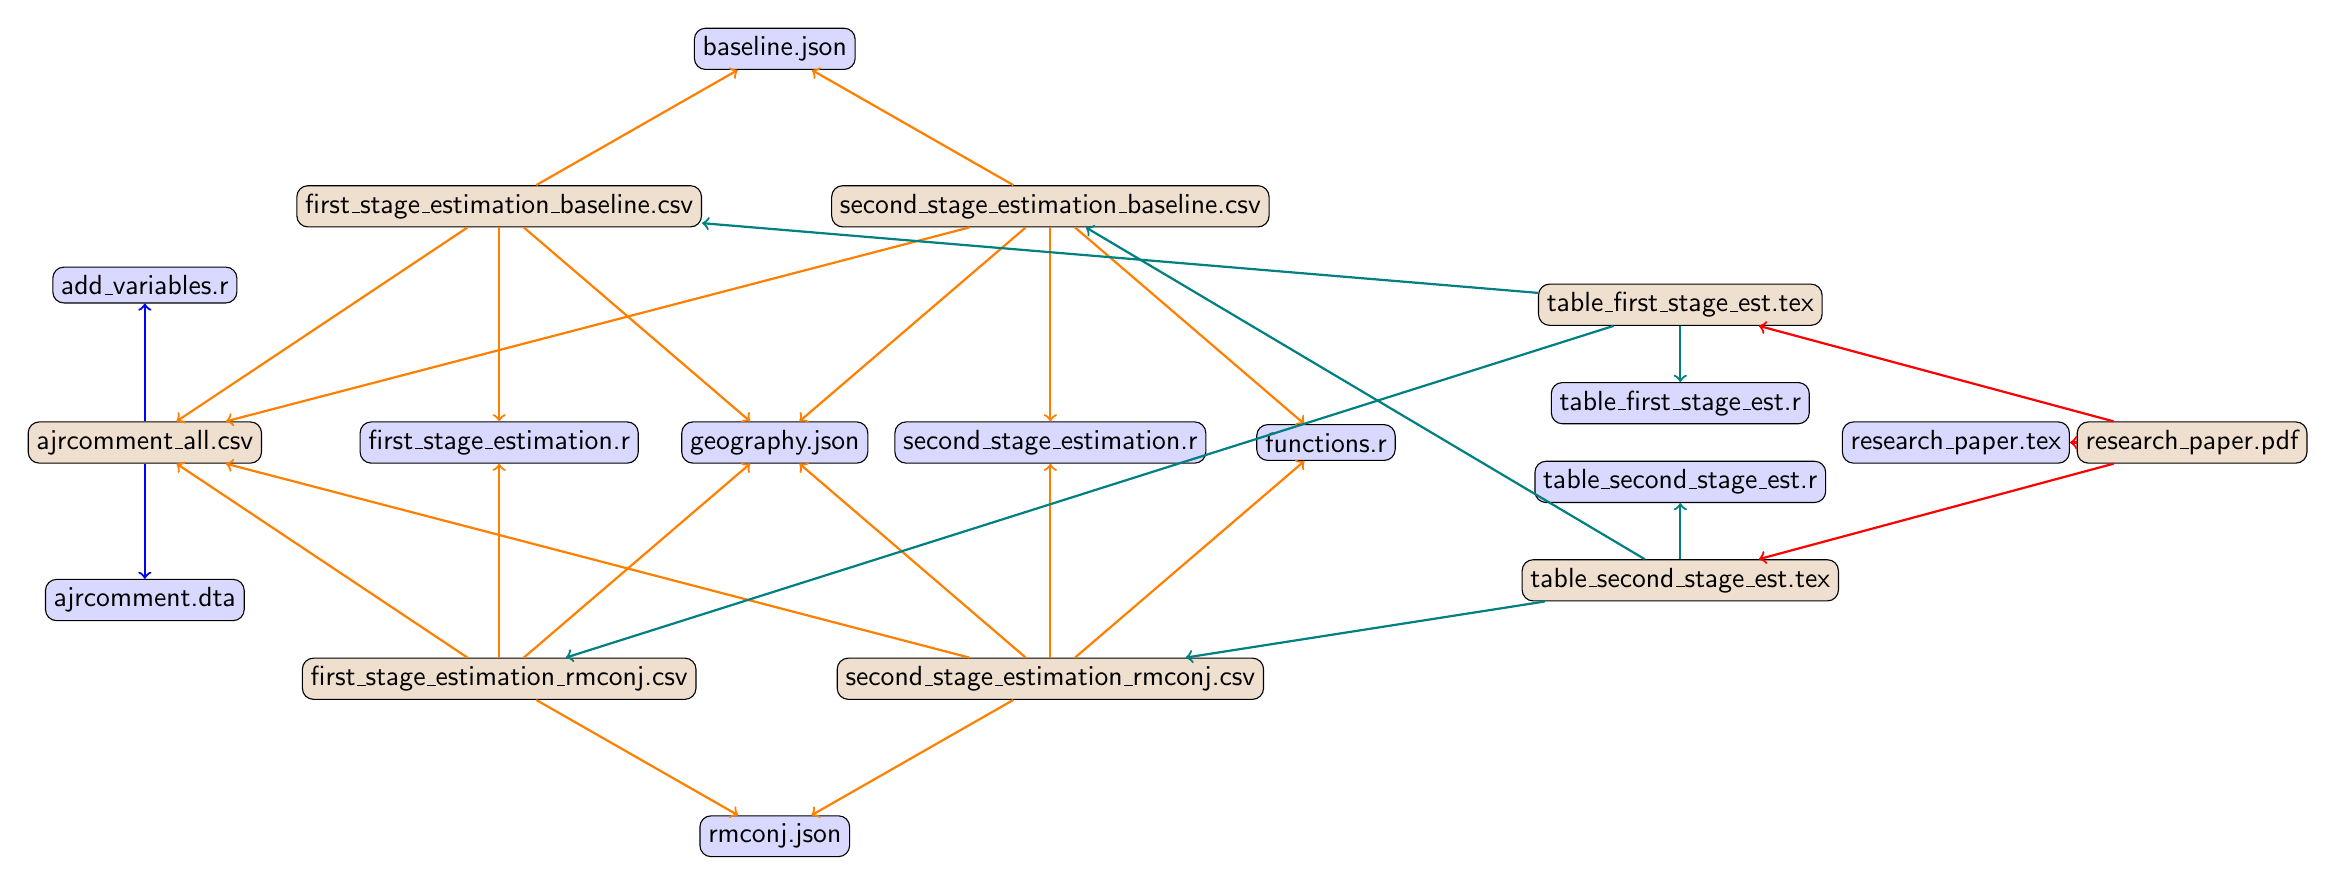
\begin{tikzpicture}[every node/.style={
    rectangle,
    rounded corners,
    inner sep=3pt,
    draw,
    fill=brown!25
}]
    %data
    \node (ajrcomment_dta) [fill=blue!15, shift={(-4, -2)}]
    {
        ajrcomment.dta
    };
    \node (add_variables_r) [fill=blue!15, shift={(-4, 2)}]
    {
        add\_variables.r
    };
    \node (ajrcomment_all_csv) [shift={(-4, 0)}]
    {
        ajrcomment\_all.csv
    };

    %analysis

    \node (geography_r) [fill=blue!15, shift={(4, 0)}]
    {
        geography.json
    };
    \node (baseline_r) [fill=blue!15, shift={(4, 5)}]
    {
        baseline.json
    };
    \node (rmconj_r) [fill=blue!15, shift={(4, -5)}]
    {
        rmconj.json
    };

    \node (functions_r) [fill=blue!15, shift={(11, 0)}]
    {
        functions.r
    };

    \node (first_stage_estimation_baseline_csv) [shift={(0.5, 3)}]
    {
        first\_stage\_estimation\_baseline.csv
    };

    \node (first_stage_estimation_rmconj_csv) [shift={(0.5, -3)}]
    {
        first\_stage\_estimation\_rmconj.csv
    };

    \node (first_stage_estimation_r) [fill=blue!15, shift={(0.5, 0)}]
    {
        first\_stage\_estimation.r
    };


    \node (second_stage_estimation_baseline_csv) [shift={(7.5, 3)}]
    {
        second\_stage\_estimation\_baseline.csv
    };

    \node (second_stage_estimation_rmconj_csv) [shift={(7.5, -3)}]
    {
        second\_stage\_estimation\_rmconj.csv
    };


    \node (second_stage_estimation_r) [fill=blue!15, shift={(7.5, 0)}]
    {
        second\_stage\_estimation.r
    };


    %final
    \node (table_first_stage_est_tex) [shift={(15.5, 1.75)}]
    {
        table\_first\_stage\_est.tex
    };

    \node (table_first_stage_est_r) [fill=blue!15, shift={(15.5, 0.5)}]
    {
        table\_first\_stage\_est.r
    };

    \node (table_second_stage_est_tex) [shift={(15.5, -1.75)}]
    {
        table\_second\_stage\_est.tex
    };

    \node (table_second_stage_est_r) [fill=blue!15, shift={(15.5, -0.5)}]
    {
        table\_second\_stage\_est.r
    };




    %paper

    \node (research_paper_tex) [fill=blue!15, shift={(19, 0)}]
    {
        research\_paper.tex
    };

    \node (research_paper_pdf) [shift={(22, 0)}]
    {
        research\_paper.pdf
    };




    %data
    \draw[->, blue, thick] (ajrcomment_all_csv) to (add_variables_r);
    \draw[->, blue, thick] (ajrcomment_all_csv) to (ajrcomment_dta);

    %analysis


    \draw[->, orange, thick] (first_stage_estimation_baseline_csv) to (geography_r);
    \draw[->, orange, thick] (first_stage_estimation_baseline_csv) to (ajrcomment_all_csv);
    \draw[->, orange, thick] (first_stage_estimation_baseline_csv) to (baseline_r);
    \draw[->, orange, thick] (first_stage_estimation_baseline_csv) to (first_stage_estimation_r);


    \draw[->, orange, thick] (first_stage_estimation_rmconj_csv) to (geography_r);
    \draw[->, orange, thick] (first_stage_estimation_rmconj_csv) to (ajrcomment_all_csv);
    \draw[->, orange, thick] (first_stage_estimation_rmconj_csv) to (rmconj_r);
    \draw[->, orange, thick] (first_stage_estimation_rmconj_csv) to (first_stage_estimation_r);

    \draw[->, orange, thick] (second_stage_estimation_baseline_csv) to (geography_r);
    \draw[->, orange, thick] (second_stage_estimation_baseline_csv) to (functions_r);
    \draw[->, orange, thick] (second_stage_estimation_baseline_csv) to (ajrcomment_all_csv);
    \draw[->, orange, thick] (second_stage_estimation_baseline_csv) to (baseline_r);
    \draw[->, orange, thick] (second_stage_estimation_baseline_csv) to (second_stage_estimation_r);

    \draw[->, orange, thick] (second_stage_estimation_rmconj_csv) to (geography_r);
    \draw[->, orange, thick] (second_stage_estimation_rmconj_csv) to (functions_r);
    \draw[->, orange, thick] (second_stage_estimation_rmconj_csv) to (ajrcomment_all_csv);
    \draw[->, orange, thick] (second_stage_estimation_rmconj_csv) to (rmconj_r);
    \draw[->, orange, thick] (second_stage_estimation_rmconj_csv) to (second_stage_estimation_r);


    %final
    \draw[->, teal, thick] (table_first_stage_est_tex) to (table_first_stage_est_r);
    \draw[->, teal, thick] (table_first_stage_est_tex) to (first_stage_estimation_baseline_csv);
    \draw[->, teal, thick] (table_first_stage_est_tex) to (first_stage_estimation_rmconj_csv);

    \draw[->, teal, thick] (table_second_stage_est_tex) to (table_second_stage_est_r);
    \draw[->, teal, thick] (table_second_stage_est_tex) to (second_stage_estimation_baseline_csv);
    \draw[->, teal, thick] (table_second_stage_est_tex) to (second_stage_estimation_rmconj_csv);


    %paper

    \draw[->, red, thick] (research_paper_pdf) to (research_paper_tex);

    \draw[->, red, thick] (research_paper_pdf) to (table_first_stage_est_tex);
    \draw[->, red, thick] (research_paper_pdf) to (table_second_stage_est_tex);


\end{tikzpicture}

\end{document}
